\chapter{Federated Learning}\label{sec:fl}
\section{Introducción}
El \textit{deep learning} ha revolucionado el campo de la \ac{IA} mediante la posibilidad de permitir a las máquinas a aprender y tomar decisiones como los humanos gracias a técnicas basadas en datos. El de desarrollo en redes de alta velocidad tales como 5G y avances en \textit{edge computing} ha permitido el desarrollo de modelos y hardware capaces de procesar grandes cantidades de datos recolectados de múltiples dispositivos. En consecuencia, la privacidad se ha convertido en una gran influencia en el diseño, llevando los esfuerzos desde el \ac{AA} centralizado al \ac{AA} distribuido. Aún así, en el \ac{AA} distribuido los costes de comunicación son inmensamente mayores que los costes de cómputo, haciendo el proceso de entrenamiento ineficiente. El \ac{FL} o \textit{Federated Learning} fue inventado para resolver estos problemas~\cite{tutorial-nuria}. En esencia, \ac{FL} es un paradigma de aprendizaje distribuido que permite a un modelo aprender a partir de datos distribuidos, sin la necesidad de estos de ser recolectados por un servidor central. Dado que los dados locales nunca abandonan los dispositivos donde son recogidos, se garantiza la privacidad de datos.

\ac{FL} ha ganado atención debido a su capacidad de resolver preocupaciones sobre la privacidad y de mejorar la eficiencia de aprendizaje distribuido. Además, es altamente escalable ya que puede soportar una gran cantidad de participantes, cada uno con su respectivas fuentes de datos. Esto puede ser realmente útil en escenarios con una generación continua de datos como puede ser el \ac{IoT}, sensores, etc. Como resultado, \ac{FL} se ha convertido en un campo importante de la \ac{IA} obteniendo el interés de investigadores, desarrolladores y científicos de datos en la comunidad del \ac{AA}. El primer caso de uso exitoso del \ac{FL} fue desarrollado por Google~\cite{mcmahan-2018} para predecir la siguiente entrada de texto del usuario en miles de dispositivos Android, mientras se mantenía los datos de los dispositivos en local. Desde entonces, el \ac{FL} se ha aplicado a un gran rango de aplicaciones en diversos campos, desde ingeniería industrial hasta el mundo de la salud~\cite{survey-nuria-2023}. 

\section{Federated Learning: ¿Qué y Por Qué?}
El \ac{AA} basado en datos domina actualmente el campo de la \ac{IA}. Desafortunadamente, la creciente demanda en término de volumen de datos y variedad ha resultado en varios problemas relacionado en la privacidad de los datos y en el procesamiento de grandes cantidades de datos. Entre ellos, los principales desafíos del \ac{AA} que llevan a la aparición del \ac{FL} están asociados con la privacidad, comunicación y acceso a los datos~\cite{tutorial-nuria}.

\begin{itemize}
    \item \textbf{Privacidad de los Datos}: en el \ac{AA} centralizado, los datos de los usuarios son recolectados y se almacenan en un servidor central, donde pueden ser vulnerables a una brecha de seguridad. Además, la creciente preocupación sobre la protección de los datos se manifiesta en el área legal. Por lo tanto, hay una urgente demanda en el desarrollo de métodos de \ac{IA} que protejan la privacidad.

    \item \textbf{Costes de Comunicación y Latencia}: en el \ac{AA} centralizado, los datos sin procesar son mandados al servidor central para ser procesados y usados para entrenar el modelo. Este intercambio de información puede ser costoso, especialmente cuando se trata con conjuntos de datos muy grandes. Además, la creciente cantidad de datos disponibles debido al drástico aumento de sensores \ac{IoT} y dispositivos móviles generando enormes cantidades de datos supone un nuevo desafío relacionado con el almacenamiento y preprocesamiento de un flujo continuo de datos.

    \item \textbf{Limitaciones al Acceso de Datos}: en algunos casos, los datos pueden ser distribuidos entre diferentes instituciones u organizaciones, haciendo complicado el acceder o compartir datos entre ellas.
\end{itemize}

Con el objetivo de resolver los desafíos previamente mencionados, \ac{FL} aparece como un paradigma de \ac{AA} distribuido enfocado en desarrollar un modelo de \ac{AA} sin explícitamente compartir ningún dato entre los participantes. Implica una red de clientes $\{C_1, C_2, \ldots, C_n \}$, que participa en dos fases principales:

\begin{enumerate}
    \item \textbf{Fase de Entrenamiento del Modelo}: cada cliente (o propietario de datos) intercambia información sin revelar ningún dato de su conjunto para entrenar de forma conjunta un modelo de \ac{AA}. Para lograr esto, cada cliente entrena un modelo local con sus datos y comparte la información de este modelo en lugar de sus datos de entrenamiento. Entonces, los modelos locales son agregados para crear un modelo global.
    \item \textbf{Fase de Inferencia}: el modelo global es aplicado a nuevas instancias de datos.
\end{enumerate}

Estos procesos pueden ser tanto síncronos como asíncronos dependiendo de la disponibilidad de los nodos y del modelo entrenado. Es importante notar que la privacidad no es la única razón para aplicar este método, ya que también se debería usar alguna estrategia para compartir los beneficios del modelo entrenado de forma colaborativa.

Una vez hemos descrito \ac{FL} como un concepto general, un escenario de \ac{FL} puede ser propuesto formalmente de la siguiente manera. Suponemos un conjunto de clientes $\{C_1, \ldots, C_n\}$ con sus respectivos conjuntos de datos de entrenamiento $\{D_1, \ldots, D_n\}$. Cada uno de estos clientes $C_i$ cuenta un con modelo local $L_i$ expresado como los parámetros $\{L_1, \ldots, L_n\}$. El \ac{FL} se enfoca en aprender un modelo global $G$, usando datos distribuidos entre clientes mediante un proceso de aprendizaje iterativo conocido como \textbf{ronda de aprendizaje}. Para ello, en cada ronda de aprendizaje $t$, cada cliente entrena su modelo local sobre sus datos locales $D_i^t$, resultando en la actualización de los parámetros locales $L_i^t$ a $\hat{L}_i^t$. Después, los parámetros globales $G^t$ son calculados agregando los parámetros locales entrenados $\{\hat{L}_1^t, \ldots, \hat{L}_n^t\}$ usando una operación fija de agregación denotada por $\Delta$. Luego los parámetros locales son actualizados con los parámetros globales agregados.
\begin{equation}
    G^t = \Delta (\hat{L}_1^t, \ldots, \hat{L}_n^t)
\end{equation}
\begin{equation}
    L^{t+1}_i \leftarrow G^t, \quad \forall i \in \{1, \ldots, n\}.
\end{equation}

Las actualizaciones entre los clientes y el servidor son repetidas durante el proceso de aprendizaje hasta que se alcanza algún criterio de parada. Así, el valor final de $G$ resumirá el conocimiento modelado en los clientes.

\section{Elementos Clave en Federated Learning}
Una vez que el \ac{FL} ha sido introducido de manera breve, podemos hablar del flujo de trabajo de un proceso de \ac{FL}. Este se compone de los siguientes pasos:
\begin{enumerate}
    \item \textbf{Entrenamiento local}: comienza con el entrenamiento local de cada uno de los modelos locales por cada uno de los clientes. Generalmente, todos estos modelos tienen una arquitectura común. Sin embargo, los aspectos relacionados con los hiperparámetros de entrenamiento (\textit{epochs}, \textit{batch size}, \textit{learning rate}) puede diferir entre clientes. En esta fase los primeros elementos aparecen de manera natural:
    \begin{itemize}
        \item \textbf{Datos Descentralizados}: los datos se encuentran distribuidos entre los distintos dispositivos o nodos, en lugar de en un mismo lugar de forma centralizada, lo cual es un beneficio cuando la privacidad es una preocupación. La distribución de los datos puede ser:
        \begin{enumerate}
            \item \textbf{Homogénea o \ac{i.i.d.}}: se asume que la distribución de datos entre los clientes es \ac{i.i.d.}, por lo que todos los clientes tienen la misma distribución.
            \item \textbf{Heterogénea o no-i.i.d.}: se asume que la distribución de datos entre los clientes no es \ac{i.i.d.}, esto es, que los datos de cada cliente sigue una distribución distinta. Formalmente se pueden distinguir entre tres tipos de heterogeneidad de la distribución de datos:
            \begin{itemize}
                \item El espacio de características de nuestros clientes es distinto pero comparten el mismo objetivo.
                \item El espacio de entradas es análogo pero el espacio de las etiquetas es distintos respecto a los mismos datos.
                \item Ambos espacios son distintos.
            \end{itemize}
        \end{enumerate}

        \item \textbf{Modelo}: el entrenamiento del modelo es realizado en los datos descentralizados, donde cada dispositivo o nodo entrena su modelo y contribuye al proceso de entrenamiento, compartiendo los pesos de su modelo local. También mejora el modelo debido a una mejor generalización, ya que el modelo puede aprender de un rango más amplio de datos.
        \item \textbf{Clientes}: estos nodos almacenan datos y entrenan modelos locales.
    \end{itemize}
    
    \item \textbf{Comunicación}: después del entrenamiento local, la comunicación permite la coordinación y agregación de las actualizaciones del modelo generadas por los participantes, permitiendo así un entrenamiento distribuido. Es un rol crucial en la protección de la privacidad y seguridad de los datos cuando se combina con varias técnicas como la \ac{DP}. Destacamos los siguientes elementos clave en este paso:
    \begin{itemize}
        \item \textbf{Planificación de Comunicaciones}: la comunicación puede ser tanto síncrona como asíncrona, dependiendo de la configuración. También puede haber un servidor central que maneja la recolección de todos los modelos locales, o puede estar distribuido a través de múltiples nodos en la red.

        \item \textbf{Protocolos de Privacidad}: pese a que no se comparten los datos de entrenamiento durante las comunicaciones en \ac{FL}, la información compartida es susceptible a brechas de privacidad o a corromper el proceso de aprendizaje en su totalidad. Por lo tanto, las comunicaciones son uno de los puntos débiles de \ac{FL} respecto a los ataques. Por esta razón es normal combinarlas con otros mecanismos de privacidad.
    \end{itemize}

    \item \textbf{Agregación}: las actualizaciones locales generadas por cada nodo son combinadas mediante un operador específico de agregación y el resultado es incorporado para actualizar y crear un modelo global entrenado. El elemento clave en este paso es el \textbf{mecanismo de agregación}, que depende en la tarea que se plantea resolver. Pese a ello, el mas común es \textbf{\ac{FedAvg}} cuando el modelo se puede expresar como un vector de pesos. En otro caso, como podría ser el \textit{clustering}, se debe de diseñar un agregador específico para combinar la información de cada nodo.
    \item \textbf{Actualización local}: el último paso consiste en actualizar los modelos locales almacenados en los distintos nodos con el nuevo modelo global. El caso más sencillo es actualizar todos los modelos locales con el modelo global. Sin embargo, hay distintas estrategias de actualización que consisten en en combinar el modelo local y el global en lugar de reemplazar el uno por el otro directamente. Estos enfoques son usados para alcanzar características tales como la personalización de los clientes a sus datos locales.
\end{enumerate}

\section{Arquitecturas de Federated Learning}
La combinación de los elementos clave genera muchas arquitecturas de \ac{FL} que definen su interrelación, ambas cliente-servidor y \textit{peer-to-peer}:
\begin{itemize}
    \item \textbf{Arquitectura Cliente-servidor}: hay un nodo que es el responsable de la coordinación y agregación de las actualizaciones del modelo que recibe el nombre de \textbf{servidor} y el resto de nodos responsables del entrenamiento de los datos locales con sus propios datos son llamados \textbf{clientes}. Es fácil de implementar pero requiere un nivel de confianza elevado en el servidor. Este grado de confianza es su principal debilidad y es por ello que es vulnerable a ataques.

    \begin{figure}[h!]
      \centering
      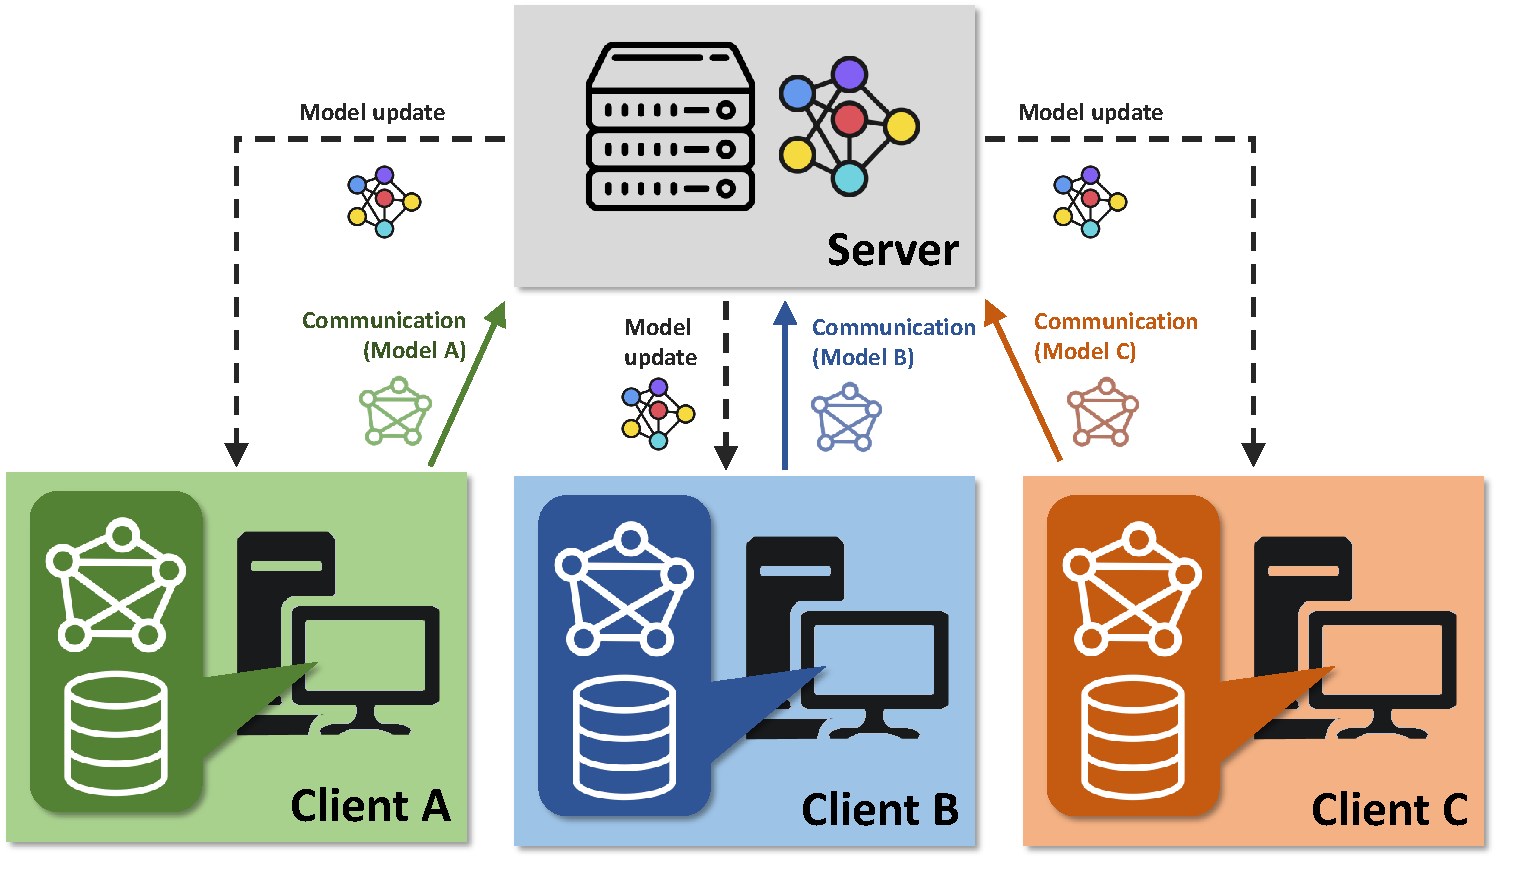
\includegraphics[width = \linewidth]{figuras/cliente-servidor.pdf}
      \caption{Representación de la arquitectura cliente-servidor en \ac{FL} con 3 clientes. Fuente: \cite{tutorial-nuria}.}
      \label{clientserver}
    \end{figure}

    \item \textbf{Arquitectura \textit{Peer-to-peer}}: todos los nodos tienen datos locales de entrenamiento y agregan las actualizaciones de los demás nodos simultáneamente. No necesita de ningún nodo coordinador del proceso de aprendizaje fijo. Es complicada de implementar, y acarrea un aumento en los costes de comunicación, pero la principal ventaja es el elevado nivel de seguridad y privacidad de datos.
\end{itemize}

La arquitectura Cliente-Servidor es la más común en \ac{FL} y consecuentemente nos referiremos a ella como la arquitectura por defecto cuando hablemos de \ac{FL}.

\section{Categorías de Federated Learning}
Hay múltiples categorías de \ac{FL} según las propiedades de los elementos clave~\cite{survey-nuria-2023}. Las siguientes categorías están hechas en términos del espacio de características ($X$), el espacio de etiquetas ($Y$) y el espacio muestral ($I$).
\begin{itemize}
    \item \textbf{\ac{HFL}}: cuando los datos forman una partición entre los clientes basado en las muestras, que significa que cada cliente es propietario de diferentes muestras de el conjunto de entrenamiento general. Formalmente, lo podemos expresar como:
    \begin{equation}
        X_i = X_j, Y_i = Y_j, I_i \ne I_j, \quad \forall D_i, D_j, i \ne j
    \end{equation}
    donde los espacios de características y etiquetas de los clientes ($i, j$) están representados por ($X_i, Y_i$) y ($X_j, Y_j$) y asumiendo que son iguales, mientras que las muestras $I_i$ y $I_j$ no coinciden. $D_i$ y $D_j$ representan los datos de los clientes $i$ y $j$. Es adecuado para entrenar modelos en datos recolectados por una gran cantidad de dispositivos similares, tales como \textit{smartphones} o dispositivos \ac{IoT}.
    \item \textbf{\ac{VFL}}: cuando los datos forman una partición entre los clientes basado en las características, lo que significa que cda cliente es propietario del mismo conjunto de muestras pero con un conjunto de características distinto. Formalmente, lo podemos expresar como:
    \begin{equation}
        X_i \ne X_j, Y_i \ne Y_j, I_i = I_j, \quad \forall D_i, D_j, i \ne j
    \end{equation}
    Es adecuado para entrenar modelos en datos recolectados por una cantidad pequeña de dispositivos con un espacio de características distinto. Por ejemplo, puede ser usado para predecir resultados médicos basado en los datos recolectados por múltiples hospitales, donde cada hospital tiene un conjunto distinto de registros.
    \item \textbf{\ac{FTL}}: cuando se transfiere conocimiento entre múltiples dominios sin que haya solapamiento entre muestras o características. Formalmente, lo podemos definir como: 
    \begin{equation}
        X_i \ne X_j, Y_i \ne Y_j, I_i \ne I_j, \quad \forall D_i, D_j, i \ne j
    \end{equation}
    En esta arquitectura, no se asume que la distribución de los datos tanto de entrenamiento como de validación sean los mismos y están definidos en el mismo espacio de características. Normalmente es usado en combinación con técnicas de \textit{fine-tuning} con modelos entrenados sobre grandes conjuntos de datos centralizados.
    \begin{figure}[h!]
        \centering
        \begin{subfigure}[]{0.3\textwidth}
            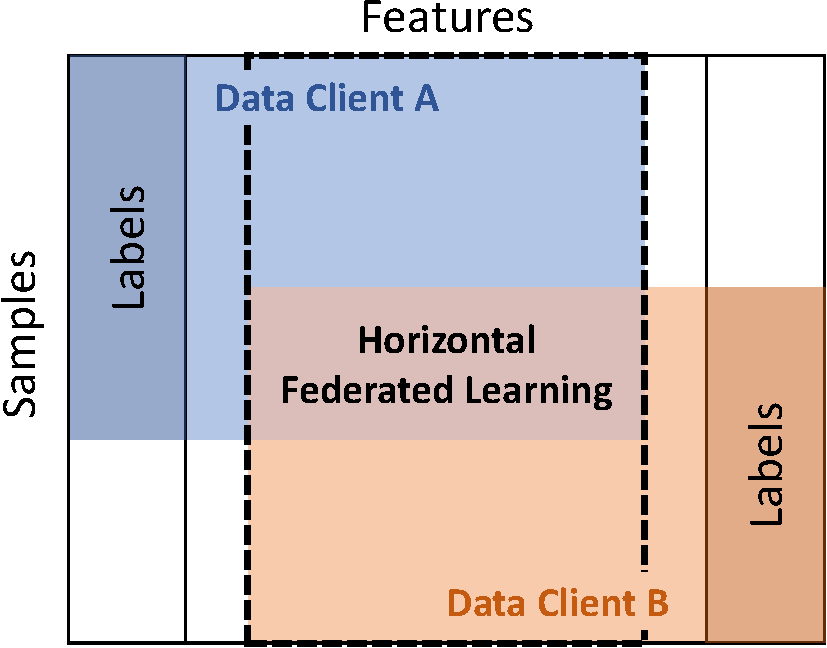
\includegraphics[width=0.95\linewidth]{figuras/hfl.pdf}
            \caption{\ac{HFL} }
            \label{fig:first}
        \end{subfigure}
        
        \hfill
        \vspace{3mm}
        
        \begin{subfigure}[]{0.3\textwidth}
            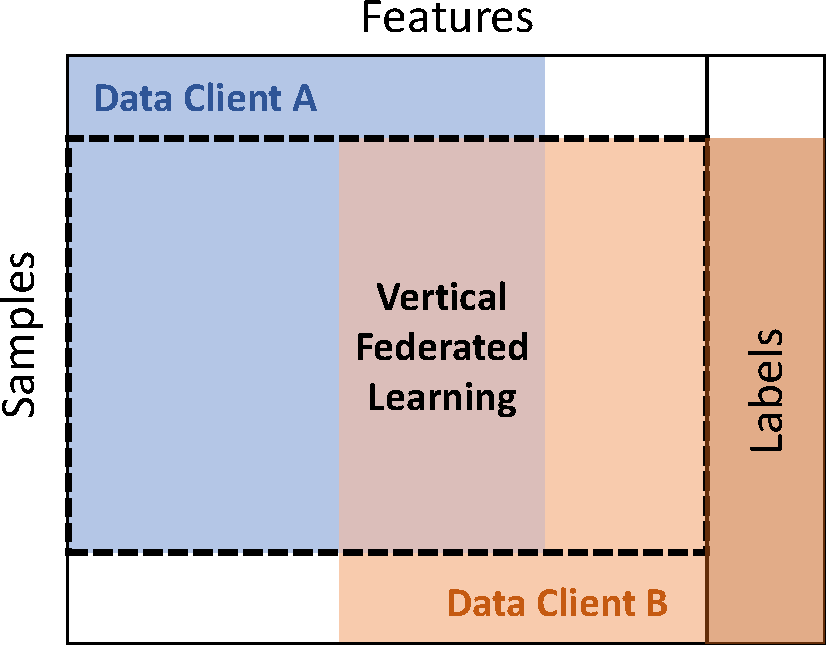
\includegraphics[width=0.95\linewidth]{figuras/vfl.pdf}
            \caption{\ac{VFL} }
            \label{fig:second}
        \end{subfigure}
        
        \hfill
        \vspace{3mm}
        
        \begin{subfigure}[]{0.3\textwidth}
            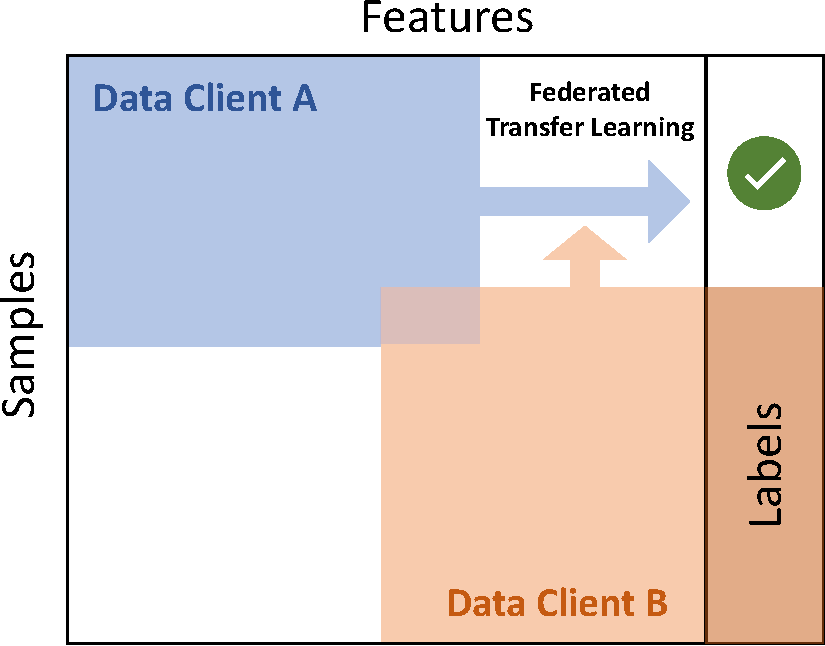
\includegraphics[width=0.95\linewidth]{figuras/ftl.pdf}
            \caption{\ac{FTL}}
            \label{fig:third}
        \end{subfigure}
        \caption{Representación de \ac{HFL}, \ac{VFL} y \ac{FTL} en una arquitectura cliente servidor en \ac{FL} \cite{yang-2019}.}
        \label{fig:architectures}
    \end{figure}

    \section{Privacidad de Datos: técnicas Avanzadas}
    El \ac{FL} ha sido desarrollado teniendo en cuenta la privacidad, esto es, los datos de los clientes se mantiene privado durante el entrenamiento del modelo. Sin embargo, es posible vulnerar estas garantías de privacidad mediante los modelos intercambiados durante el proceso de aprendizaje, ya que los modelos locales de los clientes tienden a memorizar su conjunto de entrenamiento. Un nodo malicioso puede intentar recuperar parte del conjunto de entrenamiento de otros clientes, creando así una brecha de privacidad. Es por ello, se requieren técnicas de privacidad de datos para mejorar las promesas de privacidad de un modelo de \ac{FL}. Consideramos que estas técnicas pueden ser desplegadas en múltiples elementos de la arquitectura de \ac{FL}.
    \begin{enumerate}
        \item \textbf{Computación Segura y Cifrado Homomórfico:} la  computación segura (\textit{Secure Multiparty Computation}) se concentra en asegurar comunicaciones en las rondas de \ac{FL}, principalmente en el mecanismo de agregación. Los canales de comunicación se mantienen seguros mediante el uso de cifrado homomórfico. Mientras estas técnicas evitan interferencias tanto internas como externas durante las rondas de \ac{FL}, el modelo resultante sigue siendo vulnerable a ataques que se enfoquen en extraer información a partir del modelo agregado.
        \item \textbf{Privacidad Diferencial:} la \ac{DP} es una técnica que busca mejorar la privacidad. Se enfoca en ocultar la presencia de los individuos en el modelo. Esto se logra mediante la agregación calibrada de ruido aleatorio. Cuando se aplica en \ac{FL}, la \ac{DP} se puede usar en dos momentos distintos: a) aplicar la \ac{DP} cuando se entrena el modelo localmente (\ac{DP} local), y b) en el paso de agregación creando así una versión diferencialmente privada de \ac{FedAvg}.
    \end{enumerate}

    \section{Ataques a Federated Learning}\label{sec:ataquesfl}
    El \ac{AA} es vulnerable a ataques adversarios enfocados a reducir el rendimiento del modelo o a comprometer la privacidad de datos. Así mismo, el \ac{FL} está igualmente expuesto dado que es un escenario específico de \ac{AA}~\cite{survey-nuria-2023}. Algunos de esos ataques están basados en la manipulación maliciosa de los datos de entrenamiento, que son inaccesibles en el \ac{FL}, y por lo tanto, no podemos confiar en el uso de técnicas de inspección de datos para detectar aquellos datos alterados. Es por ello que, uno de los grandes puntos débiles del \ac{FL} es el ser vulnerable a ataques adversarios que pueden comprometer la integridad del modelo de aprendizaje o la privacidad de los datos.

    Es por esto que esta sección se centrará en dar una serie de taxonomías en ataques de adversarios sobre el \ac{FL}.

    \subsection{Escenarios del Ataque}
    Los escenarios del ataque en \ac{AA} son una representación estructurada de la información, tales que permiten identificar y definir potenciales problemas de seguridad. Pueden ser definidos en términos de la información disponible y en el rango de acción del atacante. En este contexto, definimos los siguientes conjuntos de términos mutuamente exclusivos que nos permiten definir un modelo de ataque en \ac{FL}.

        \paragraph{Atacante externo vs. Interno:} uno de los elementos clave de cualquier sistema distribuido es la comunicación entre distintas partes. La comunicación es muy vulnerable, ya que puede ser comprometida por agentes externos al sistema de aprendizaje, que son conocidos como atacantes externos o \textit{outsiders}. Cuando el ataque es realizado por uno de los participantes del sistema distribuido, ya sea uno o más clientes, o incluso el servidor, se conoce como atacante interno o \textit{insider}. Claramente, el alcance de los dos ataques es bastante diferente. Los ataques internos son son más dañinos y pueden estar enfocados a modificar el comportamiento del modelo o a inferir información de otros clientes, mientras que los ataques externos normalmente solo se enfocan a inferir información sobre los datos o del modelo resultante. Nos enfocamos en los ataques internos, de los que podemos destacar las siguientes categorías:
        \begin{itemize}
            \item \textbf{Ataques Bizantinos}: consisten en mandar actualizaciones arbitrarias al servidor, comprometiendo el rendimiento del modelo global.
            \item \textbf{Ataques sibilino}: consisten en ataques colaborativos, ya sea mediante la agrupación de varios ataques o simulando clientes ficticios con el fin de ser más dañinos.
        \end{itemize}
        
        \paragraph{Cliente vs. Servidor:} respecto a los ataques internos, en el \ac{HFL} es normal diferenciar entre dos tipos de ataques, dependiendo si se están llevando a cabo por un cliente o por un servidor. La principal diferencia recae en la cantidad de información disponible. Mientras que los ataques realizados por clientes solo tienen información de uno o varios clientes, el servidor tiene información sobre la arquitectura del modelo y las actualizaciones de los clientes en cada ronda de aprendizaje. Incluso, en implementaciones criptográficas del medio de comunicación entre clientes y servidor, el servidor tiene más información que los clientes, ya que es el único con suficiente conocimiento para descifrar los modelos.
        
        \paragraph{Conocimiento del Atacante:} en escenarios centralizados, el atacante de caja blanca tiene acceso completo al modelo objetivo, incluyendo su arquitectura, los parámetros y el estado interno. Por el otro lado, el atacante de caja negra no tiene ningún acceso al modelo objetivo y además, puede tener algún tipo de información adicional sobre la arquitectura del modelo objetivo o su procedimiento de entrenamiento. Estas dos clasificaciones de conocimiento del atacante son demasiado generales para representar cualquier tipo de atacante, ya que no hay un término medio para considerar atacantes cuyo conocimiento en el caso de caja negra sea demasiado restringido o que en el caso de caja blanca no esté lo suficientemente acotado. Para ello, en~\cite{truex-2021} se introdujo un atacante de caja gris, que consiste en un atacante de caja negra con algún conocimiento estadístico específico no público que afecta a su víctima. En el \ac{FL}, los atacantes de caja blanca, caja gris o caja negra pueden ser cualquier nodo, ya sea los clientes o el servidor. La mayoría de los ataques están relacionados con los datos pertenecientes a los clientes y a la comunicación entre el servidor federado y los clientes. Por lo tanto, también se requiere incluir información acerca del proceso de entrenamiento federado y de los datos privados de los clientes. Por lo tanto~\cite{survey-nuria-2023} define la siguiente clasificación de conocimiento de los atacantes adaptada a \ac{HFL} y \ac{VFL}:

        En un sistema estándar de \ac{HFL}, el atacante que tiene un cliente tiene \textbf{conocimiento por parte del cliente}:
        \begin{itemize}
            \item Acceso de caja blanca al modelo agregado.
            \item Acceso de caja blanca al modelo local entrenado por el cliente.
            \item Acceso al conjunto de datos del cliente.
        \end{itemize}

        Si el atacante tiene acceso a los datos locales de otros clientes o sus etiquetas, tiene \textbf{conocimiento extra por parte del cliente}.

        Si el atacante es propietario del servidor federado tiene \textbf{conocimiento por parte del servidor}:
        \begin{itemize}
            \item Acceso de caja blanca al modelo agregado después de cada ronda de comunicación.
            \item Acceso de caja blanca a los modelos entrenados por los clientes o, alternativamente, acceso a sus gradientes.
            \item Los identificadores de los clientes agregados en cada ronda de comunicación.
            \item Las etiquetas de cada cliente y, opcionalmente, el tamaño de su conjunto de datos.
        \end{itemize}

        En sistema estándar de \ac{VFL}, el atacante que tiene a un cliente tiene \textbf{conocimiento por parte del grupo}:
        \begin{itemize}
            \item Acceso de caja blanca a los parámetros relacionados con las características del cliente.
            \item Acceso al conjunto privado del cliente.
            \item El resultado parcial de los parámetros, cuando se solicita inferencia.
        \end{itemize}

        Además, si el atacante tiene información relacionada con las características de otros clientes, tiene \textbf{conocimiento extra por parte del grupo}.

        Un atacante que tiene al coordinador de aprendizaje de un sistema de \ac{VFL} tiene \textbf{conocimientos del lado de terceros}:
        \begin{itemize}
            \item Los gradientes compartidos por cada cliente.
            \item La pérdida calculada.
            \item Los resultados parciales de cada cliente, cuando se solicita inferencia.
        \end{itemize}

        Si solo un subconjunto de los conocimientos especificados está disponible, entonces el atacante tiene \textbf{conocimiento parcial}, y especificamos el subconjunto del conocimiento. Además, se espera que las defensas reduzcan el conocimiento del atacante, por lo tanto, en presencia de un método de defensa el atacante se supone que tiene \textbf{conocimiento parcial}.

        Tanto en \ac{HFL} como en \ac{VFL}, si el atacante solo tiene acceso a los resultados del modelo federado, entonces tiene \textbf{conocimiento del lado externo}.
        
        \paragraph{Honesto pero curioso vs. Malicioso:} un atacante malicioso (o activo) intenta interferir en el proceso de entrenamiento del modelo con el objetivo corromper el modelo, por ejemplo, dañando su rendimiento o inyectando una tarea secundaria. Por el otro lado, un atacante honesto pero curioso (o pasivo) no interfiere en el proceso de entrenamiento y sigue los protocolos de aprendizaje, pero intenta obtener información privada sobre otros clientes a partir de la información recibida.

        
        \paragraph{Colusión vs. no Colusión:} la amenaza de colusión se basa en el hecho de que el atacante que controle más clientes tiene más poder en un sistema distribuido. Hay dos tipos de colusión:
        \begin{enumerate}
            \item \textbf{Servidor-Participantes}: el atacante controla algunos participantes benignos y el servidor, e intenta inferir información sobre el resto de clientes.
            \item \textbf{Participante-Participante}: el atacante controla una fracción de clientes benignos e intenta inferir información sobre otros clientes, el servidor o intenta dañar el modelo.
        \end{enumerate}
\end{itemize}

\subsection{Ataques Adversarios en \textit{Federated Learning}: taxonomías}
Los ataques adversarios representan uno de los problemas más difíciles en \ac{FL}, debido a la alta cantidad de ataques existentes y a la dificultad de defenderse ante ellos. Además, la naturaliza distribuida del \ac{FL} lo hace vulnerable a una gran variedad de ataques adversarios con distintos objetivos y usando distintas maneras de alcanzar estos objetivos. Es por ello que es difícil establecer una taxonomía común para todos los los tipos de ataques adversarios. Es por ello que en \cite{survey-nuria-2023} se propone primero una amplia clasificación diferenciando entre:
    
\begin{itemize}
    \item \textbf{Ataques al modelo federado}, que buscan cambiar su comportamiento.
    \item \textbf{Ataque a la privacidad de datos}, cuyo propósito es inferir información sensible del proceso de aprendizaje.
\end{itemize}

\begin{figure}[h!]
    \centering
    \begin{center}
\resizebox{0.5\textwidth}{!}{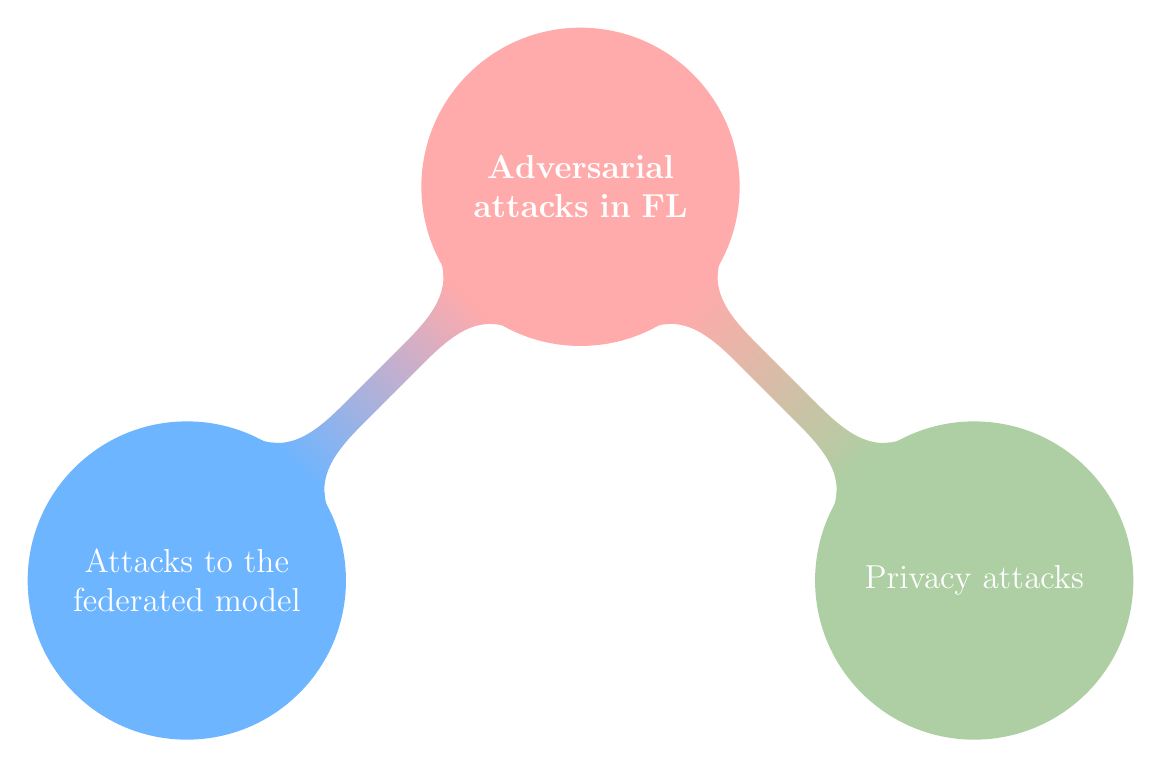
\begin{tikzpicture}[mindmap,
  level 1 concept/.append style={level distance=130,sibling angle=30},
  extra concept/.append style={color=blue!50,text=black}]

    \definecolor{rojo_pastel}{HTML}{FFABAB}
    \definecolor{azul_pastel}{HTML}{6EB5FF}
    \definecolor{verde_pastel}{HTML}{ADCFA3}


  % Applied area: computer science and its subfields
 
  \begin{scope}[mindmap, concept color=rojo_pastel, text=white]
    \node [concept] (root) at (0, 0) {\textbf{Adversarial attacks in FL}};
  \end{scope}

  % Applied area: theoretical physics and its subfields

  \begin{scope}[mindmap, concept color=azul_pastel, text=white]
    \node [concept] (property) at (-5, -5) {Attacks to the federated model};
  \end{scope}
  
  
  \begin{scope}[mindmap, concept color=verde_pastel, text=white]
    \node [concept] (feature) at (5, -5) {Privacy attacks};
  \end{scope}
  
  
    \path (root) to[circle connection bar switch color=from (rojo_pastel) to (azul_pastel)] (property);
    \path (root) to[circle connection bar switch color=from (rojo_pastel) to (verde_pastel)] (feature);

\end{tikzpicture}}
\end{center}
    \caption{Categorización de los ataques adversarios en dos grandes categorías. Fuente: \cite{survey-nuria-2023}.}
    \label{fig:main_categorisation}
\end{figure}
En este trabajo nos interesaremos sobretodo en los \textbf{ataques al modelo federado} y son en los que haremos hincapié en lo que sigue del trabajo.

\subsection{Ataques Adversarios al Modelo Federado}\label{sec:adversarialattacks}
Una de las principales limitaciones del \ac{FL}, y más concretamente el \ac{HFL}, en términos de ataques adversarios, es que los clientes tienen la habilidad de dañar el modelo mediante el envío de actualizaciones envenenadas, mientras que el servidor no puede inspeccionar los datos de entrenamiento almacenados por los clientes. Esto hace que los ataques adversarios al modelo federado sean uno de los retos más importantes en el \ac{FL}.

\textbf{\begin{figure}[!t]
\centering
\usetikzlibrary{mindmap,backgrounds,shapes.misc}

\begin{center}
\resizebox{0.9\textwidth}{!}{
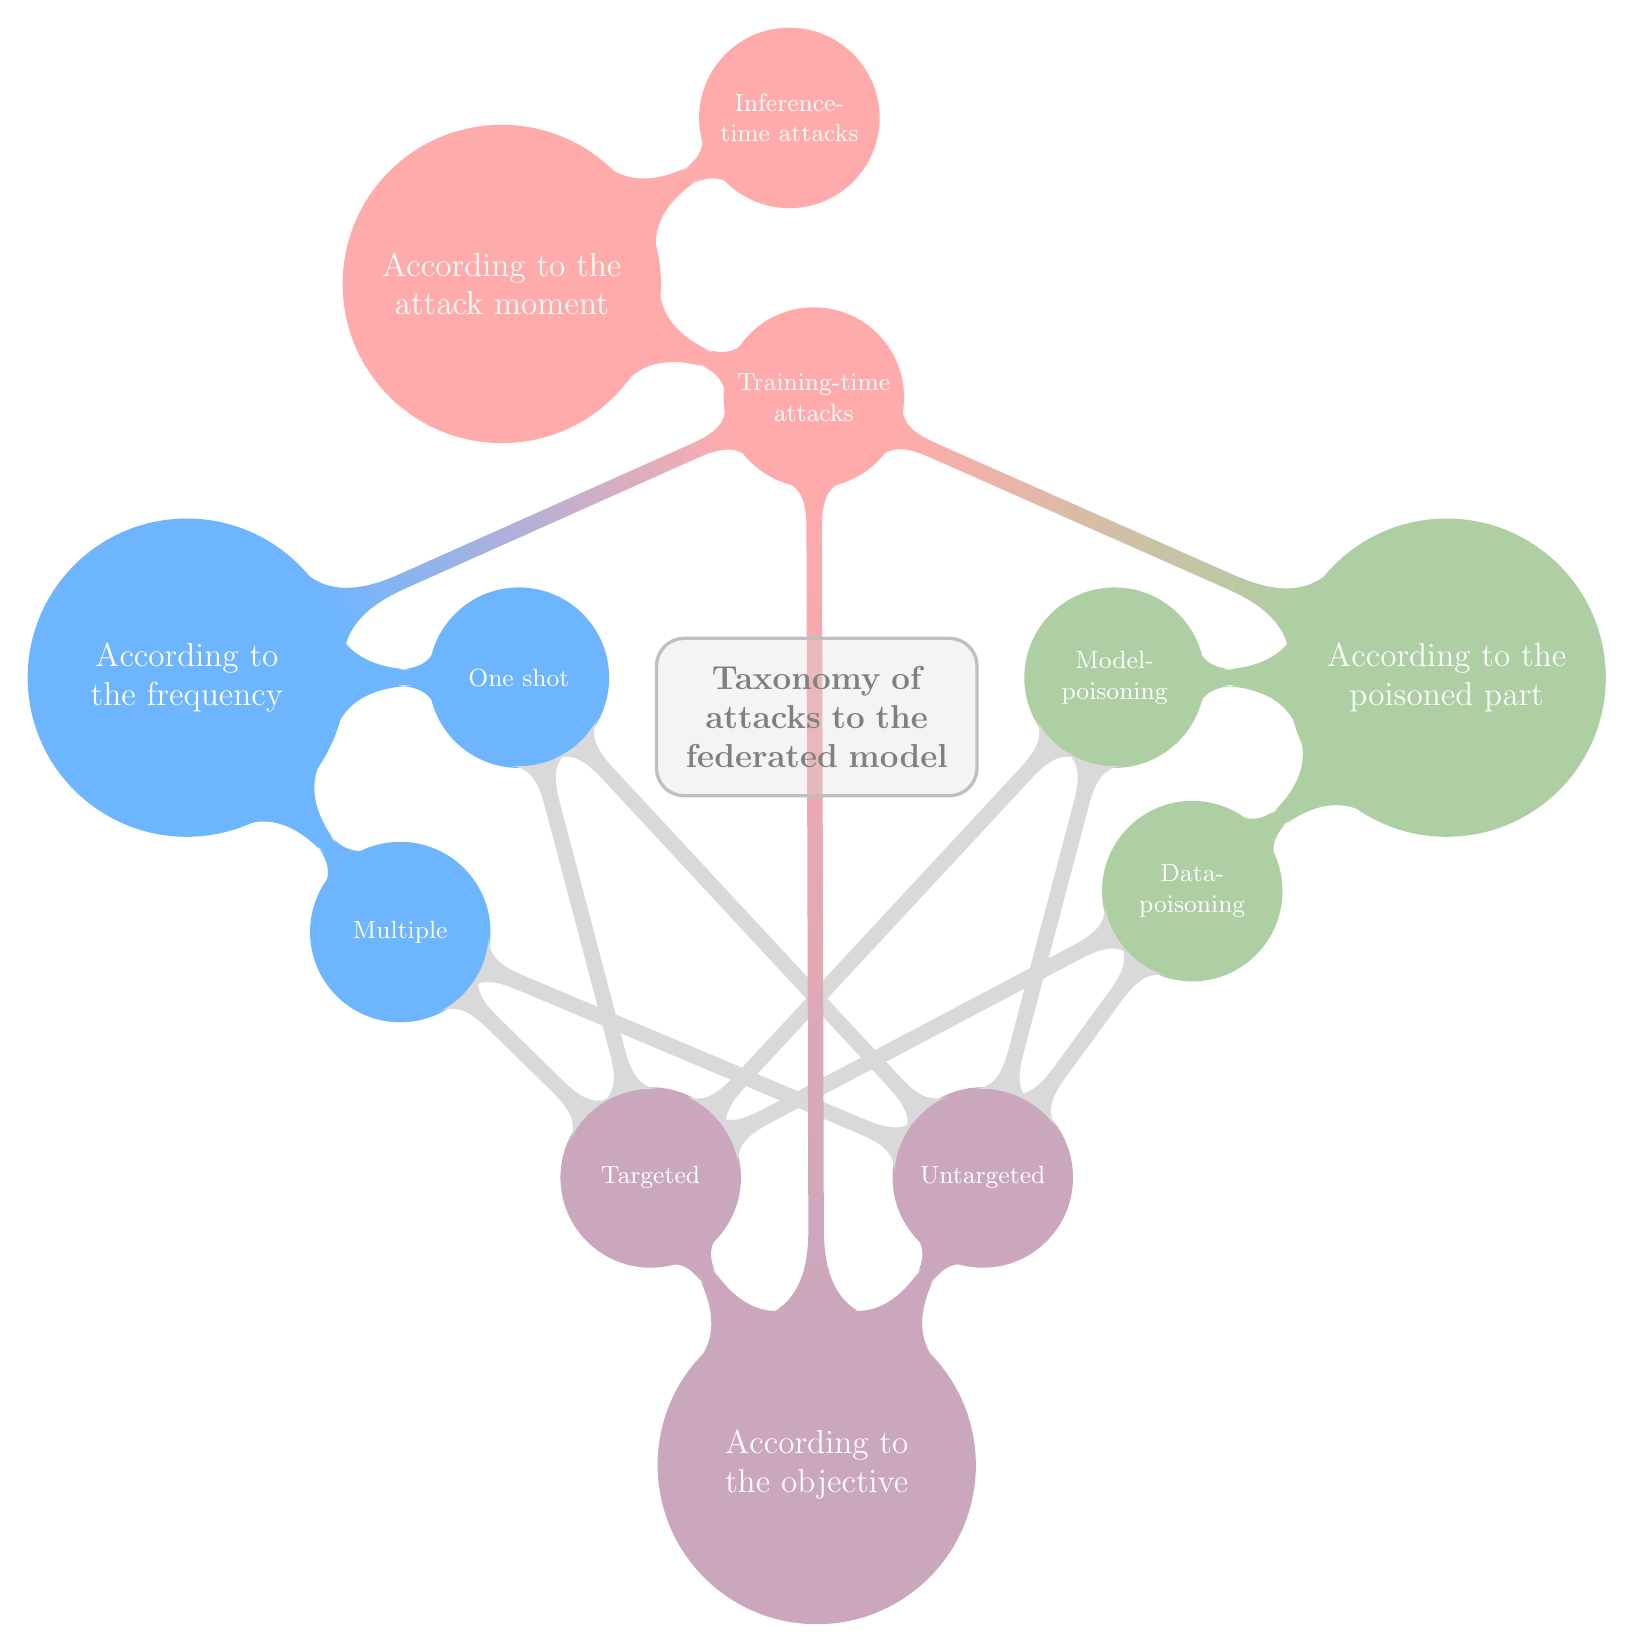
\begin{tikzpicture}[mindmap,
  level 1 concept/.append style={level distance=130,sibling angle=30},
  extra concept/.append style={color=morado_pastel!50,text=black}]

    \definecolor{rojo_pastel}{HTML}{FFABAB}
    \definecolor{azul_pastel}{HTML}{6EB5FF}
    \definecolor{verde_pastel}{HTML}{ADCFA3}
    \definecolor{morado_pastel}{HTML}{CAA7BD}

    

  % Applied area: computer science and its subfields

  \begin{scope}[mindmap, concept color=rojo_pastel, text=white]
    \node [concept] at (-4, 3) {According to the attack moment}
      child [grow=30, level distance=120] {node [concept] (test) {Inference-time attacks}}
      child [grow=-20, level distance=120] {node [concept] (training) {Training-time attacks}};
  \end{scope}

  % Applied area: theoretical physics and its subfields

  \begin{scope}[mindmap, concept color=azul_pastel,text=white]
    \node [concept] (frequency) at (-8,-2) {According to the frequency}
      child [grow=-50, level distance=120]
        {node [concept] (mul) {Multiple}}
      child [grow=0, level distance=120] 
        {node [concept] (one) {One shot}};
  \end{scope}
  
  
    \begin{scope}[mindmap, concept color=morado_pastel,text=white]
    \node [concept] (objective) at (0,-12) {According to the objective}
      child [grow=120, level distance=120]
        {node [concept] (tar) {Targeted}}
      child [grow=60, level distance=120] 
        {node [concept] (untar) {Untargeted}};
  \end{scope}

    \begin{scope}[mindmap, concept color=verde_pastel,text=white]
    \node [concept] (part) at (8,-2) {According to the poisoned part}
      child [grow=220, level distance=120]
        {node [concept] (data) {Data-poisoning}}
      child [grow=180, level distance=120] 
        {node [concept] (model) {Model-poisoning}};
  \end{scope}



  % Connections of researchers to applied subfields


    \path (one) to[circle connection bar switch color=from (black!15) to (black!15)] (tar);
    \path (one) to[circle connection bar switch color=from (black!15) to (black!15)] (untar);
    \path (mul) to[circle connection bar switch color=from (black!15) to (black!15)] (tar);
    \path (mul) to[circle connection bar switch color=from (black!15) to (black!15)] (untar);
    \path (data) to[circle connection bar switch color=from (black!15) to (black!15)] (tar);
    \path (data) to[circle connection bar switch color=from (black!15) to (black!15)] (untar);
    \path (model) to[circle connection bar switch color=from (black!15) to (black!15)] (tar);
    \path (model) to[circle connection bar switch color=from (black!15) to (black!15)] (untar);

    
    \path (training) to[circle connection bar switch color=from (rojo_pastel) to (azul_pastel)] (frequency);
    \path (training) to[circle connection bar switch color=from (rojo_pastel) to (morado_pastel)] (objective);
    \path (training) to[circle connection bar switch color=from (rojo_pastel) to (verde_pastel)] (part);
    
     \node[rectangle, draw, fill=black!15, fill opacity=0.3,draw = lightgray, rounded corners = 10pt, text opacity = 1, text = gray, text width=4cm, minimum height = 2cm] (r) at (0,-2.5) {\large \textbf{Taxonomy of attacks to the federated model}};


\end{tikzpicture}}
\end{center}

\caption{Representación de las taxonomías de los ataques según varios criterios. Los enlaces grises representan la posibilidad de combinar dos categorías. Fuente: \cite{survey-nuria-2023}.}
\label{fig:attacks_to_model}
\end{figure}}

En general, estos ataques son realizados por clientes y por tanto cuentan con características de caja blanca ya que el atacante tiene conocimiento por parte del cliente, ya sea que haya uno o varios clientes adversarios (atacantes). En algunas situaciones se considera que los atacantes tienen más información de caja blanca, como puede ser el método de agregación usado por el servidor, lo cual no es algo realista, por lo que \cite{survey-nuria-2023} solo tiene en cuenta aquellos ataques que requieren información del cliente adversario.

Dentro de esta amplia categoría, se propone una taxonomía que clasifica un abanico de ataques según diferentes criterios. Así, cada tipo de ataque en la literatura pertenece a cuatro categorías distintas, una para cada criterio.

\paragraph{Taxonomía según el momento del ataque}\mbox{}\\
Esta taxonomía representa en que momento se realiza el ataque, lo cual determina completamente la capacidad de influenciar al modelo federado. Clasificamos en dos tipos de ataques:
\begin{itemize}
    \item \textbf{Ataques durante entrenamiento}: esta fase incluye la recolección de los datos la preparación de estos para el entrenamiento. Son los ataques más comunes en la literatura ya que tienen la capacidad de alterar el modelo federado que es entrenado e inferir información sobre los datos de entrenamiento.
    \item \textbf{Ataques durante inferencia}: se llevan a cabo durante la fase de inferencia cuando el modelo ya ha sido entrenado. Se llaman también ataques exploratorios. Generalmente no pretenden alterar el modelo entrenado sino producir predicciones erróneas o recolectar información sobre las características del modelo.
\end{itemize}

\paragraph{Taxonomía según el objetivo del ataque}\mbox{}\\
Este es el criterio más usado en la literatura y por tanto el más importante a la hora de clasificar estos ataques. Podemos denotar dos grandes grupos de ataques según el objetivo del ataque:
\begin{enumerate}
    \item \textbf{Ataques de \textit{Backdoor}}: el principal objetivo es inyectar una tarea secundaria o \textit{backdoor} en el modelo. Es decir, un ataque de este tipo será exitoso si logra mantener el rendimiento de la tarea original mientras inyecta otra tarea. Estos ataques son muy silenciosos, ya que no suelen afectar al rendimiento de la tarea original, haciéndolos difíciles de detectar. Pese a que no suponen un riesgo a la principal tarea de aprendizaje, si representan un peligro para la integridad del sistema, ya que el atacante se aprovecha de la infraestructura federada para realizar alguna acción secundaria, logrando así una brecha de seguridad. La naturaleza de estos ataques es amplia, debido a la inmensa cantidad de tareas secundarias posibles. Se presenta una taxonomía basada en diferentes criterios:
    \begin{itemize}
        \item \textbf{Estrategias basadas en Entrada-Instancia}: el objetivo es que el modelo etiqueta ciertas entradas concretas con una etiqueta concreta diferente de la original. Por ejemplo, en un sistema de reconocimiento facial que permite el acceso a una casa, identificar cinco personas de la entrada original, quienes originalmente no tenían acceso (etiqueta negativa como etiqueta original) como personas que sí tienen acceso (etiqueta positiva como etiqueta objetivo).
        \item \textbf{Estrategias basadas en patrones}: el objetivo es que el modelo asocia un patrón particular con una etiqueta en concreto. Por ejemplo, en el ejemplo anterior, permitir acceso a cualquier persona que lleve una corbata de puntos. De esta manera, el sistema identificaría el patrón ``corbata de puntos`` con la etiqueta objetivo (etiqueta positiva). En la práctica, se escoge un patrón simple como una cruz o una marca parecida para la asociación.
        

        Además, estos ataques también se pueden clasificar según diferentes criterios sobre el patrón inyectado.
        \textbf{\begin{figure}[!t]
            \centering
            \begin{center}
\resizebox{0.8\textwidth}{!}{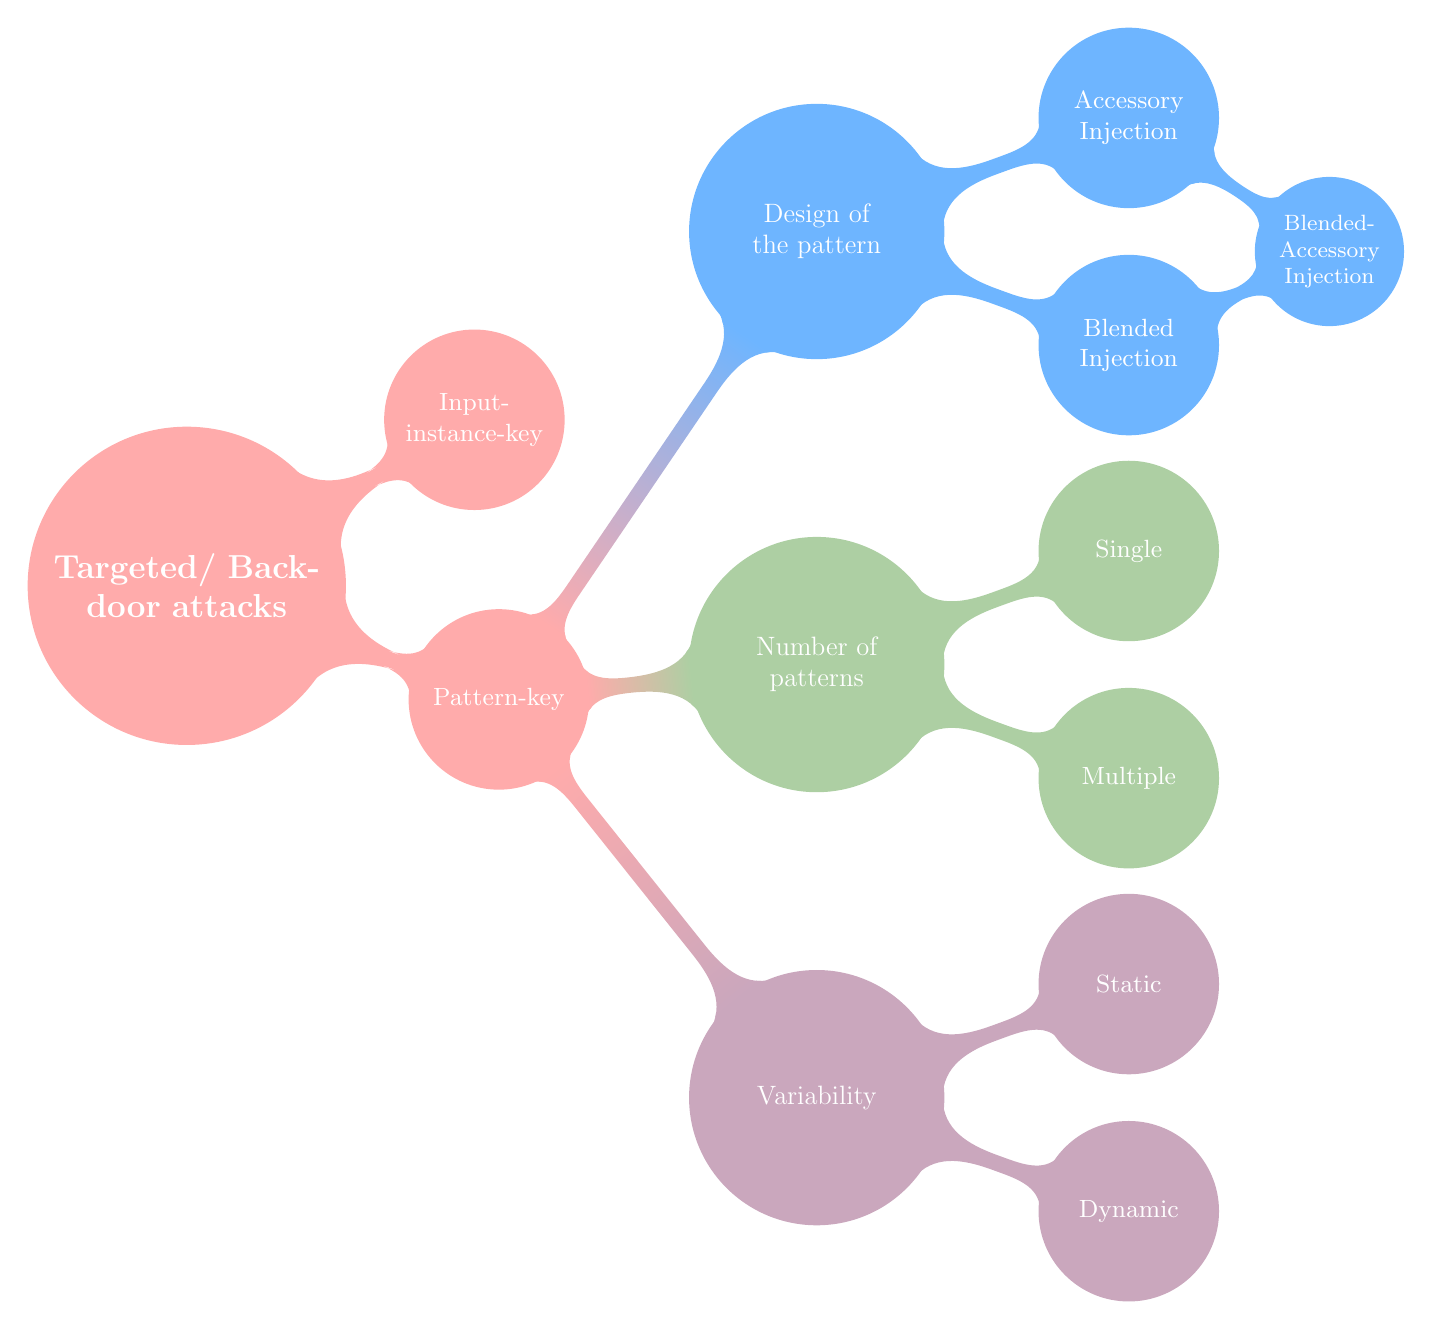
\begin{tikzpicture}[mindmap,
  level 1 concept/.append style={level distance=130,sibling angle=30},
  extra concept/.append style={color=verde_pastel!50,text=black}]


    \definecolor{rojo_pastel}{HTML}{FFABAB}
    \definecolor{azul_pastel}{HTML}{6EB5FF}
    \definecolor{verde_pastel}{HTML}{ADCFA3}
    \definecolor{morado_pastel}{HTML}{CAA7BD}

  \begin{scope}[mindmap, concept color=rojo_pastel, text=white]
    \node [concept] at (-20, 3) {\textbf{Targeted/ Backdoor attacks}}
      child [grow=30, level distance=120] {node [concept] (input) {Input-instance-key}
      }
      child [grow=-20, level distance=120] {node [concept] (pattern) {Pattern-key}};
  \end{scope}

  % Applied area: theoretical physics and its subfields

  \begin{scope}[mindmap, concept color=azul_pastel,text=white]
    \node [concept, scale=0.8] (design) at (-12,7.5) {Design of the pattern}
      child [grow=-20, level distance=120]
        {node [concept] (blended) {Blended Injection}
        child [grow=25, level distance=80] {node [concept] (mix) {Blended-Accessory Injection}}
        }
      child [grow=20, level distance=120] 
        {node [concept] (accessory) {Accessory Injection}};
  \end{scope}
  
  
    \begin{scope}[mindmap, concept color=verde_pastel, text=white]
    \node [concept, scale=0.8] (number) at (-12, 2) {Number of patterns}
      child [grow=20, level distance=120] {node [concept] (single) {Single}
      }
      child [grow=-20, level distance=120] {node [concept] (multiple) {Multiple}};
  \end{scope}
  
      \begin{scope}[mindmap, concept color=morado_pastel, text=white]
    \node [concept, scale=0.8] (var) at (-12, -3.5) {Variability}
      child [grow=20, level distance=120] {node [concept] (static) {Static}
      }
      child [grow=-20, level distance=120] {node [concept] (dyn) {Dynamic}};
  \end{scope}

    \path (pattern) to[circle connection bar switch color=from (rojo_pastel) to (azul_pastel)] (design);
    \path (mix) to[circle connection bar switch color=from (azul_pastel) to (azul_pastel)] (accessory);
    \path (pattern) to[circle connection bar switch color=from (rojo_pastel) to (verde_pastel)] (number);
    \path (pattern) to[circle connection bar switch color=from (rojo_pastel) to (morado_pastel)] (var);
\end{tikzpicture}}
    
\end{center}
            \caption{Representación de la taxonomía de ataques de \textit{Backdoor}. Fuente: \cite{survey-nuria-2023}.}
            \label{fig:backdoor_attacks}
        \end{figure}}

        Según el diseño del patrón se puede clasificar de la siguiente manera:
        \begin{itemize}
            \item \textbf{Estrategia de Inyección Mezclada}: esta estrategia generas instancias \textit{backdoor} mezclando una entrada benigna con un patrón usando un ratio de mezcla. El patrón puede ser cualquier imagen, o incluso patrones aleatorios. La principal limitación es que el mecanismo requiere modificar la mezcla completa durante entrenamiento y evaluación, lo que no tiene por qué ser viable.
            \item \textbf{Estrategia de Inyección con Accesorio}: este ataque aparece como solución la estrategia de inyección mezclada y propone generar imágenes \textit{backdoor} añadiendo patrones sobre algunas regiones de las imágenes originales. Es el equivalente a vestir un accesorio en la vida real.
            \item \textbf{Estrategia de inyección mezclada con accesorio}: combina ambas estrategias mencionadas anteriormente.
        \end{itemize}
        

        Según la cantidad de patrones:
        \begin{itemize}
            \item \textbf{Ataque de Patrón Único}: se refiere a cuando todos los clientes adversarios inyectan el mismo patrón al modelo. Tienden a tener más éxito ya que con un ataque colectivo con el mismo objetivo, pero a la vez son más fáciles de identificar en el servidor.
            \item \textbf{Ataque \textit{Multi-Backdoor}}: está compuesto de varios clientes adversarios coordinados (sibilino), donde cada cliente inyecta un patrón diferente o una parte de un patrón común en el modelo. Son más difíciles de detectar en el servidor debido a la distribución del patrón entre clientes. Sin embargo, es más complicado para los clientes inyectar tareas de \textit{backdoor} en el moddelo debido a la diversidad de las tareas secundarias.
        \end{itemize}
        

        Según la variabilidad del patrón a lo largo del tiempo:
        \begin{itemize}
            \item \textbf{Ataque estático}: cuando el patrón se mantiene a lo largo del tiempo pese a la frecuencia del ataque. Esta situación es la más común.
            \item \textbf{Ataque dinámico}: el patrón cambia a lo largo del tiempo, lo cual se convierte en un reto tanto para las defensas, ya que el patrón a identificar cambia, y para los clientes adversarios, que sufren un aumento en coste computacional para adaptar las nuevas tareas secundarias.
        \end{itemize}

    \end{itemize}


    \item \textbf{Ataques sin objetivo}: en contraposición con los ataques de \textit{backdoor}, el único objetivo de los ataques sin objetivo es reducir el rendimiento del modelo en la tarea original. El escenario más extremo es conocido como \textbf{ataques Bizantinos}, en el que los clientes adversarios comparten actualizaciones generadas aleatoriamente o entrenadas sobre datos modificados de manera aleatoria, generando por lo tanto también actualizaciones aleatorias. Claramente, estos ataques son menos silenciosos que los ataques de \textbf{backdoor} y por lo tanto pueden ser detectados simplemente midiendo el rendimiento del modelo local en el servidor, aunque a veces es difícil distinguirlos de clientes con distribuciones de datos bastantes particulares.
\end{enumerate}


\paragraph{Taxonomía según la parte del esquema envenenada}\mbox{}\\
La mayoría de ataques durante el entrenamiento están basados en envenenar la información del cliente con la intención de corromper el modelo global. Dependiendo qué parte de la información del cliente se envenene, podemos diferenciar entre envenenamiento de datos y envenenamiento de modelo, aunque nos referiremos a ambos como ataques de envenenamiento.
\begin{figure}[h!]
    \centering
    \begin{center}
\resizebox{0.8\textwidth}{!}{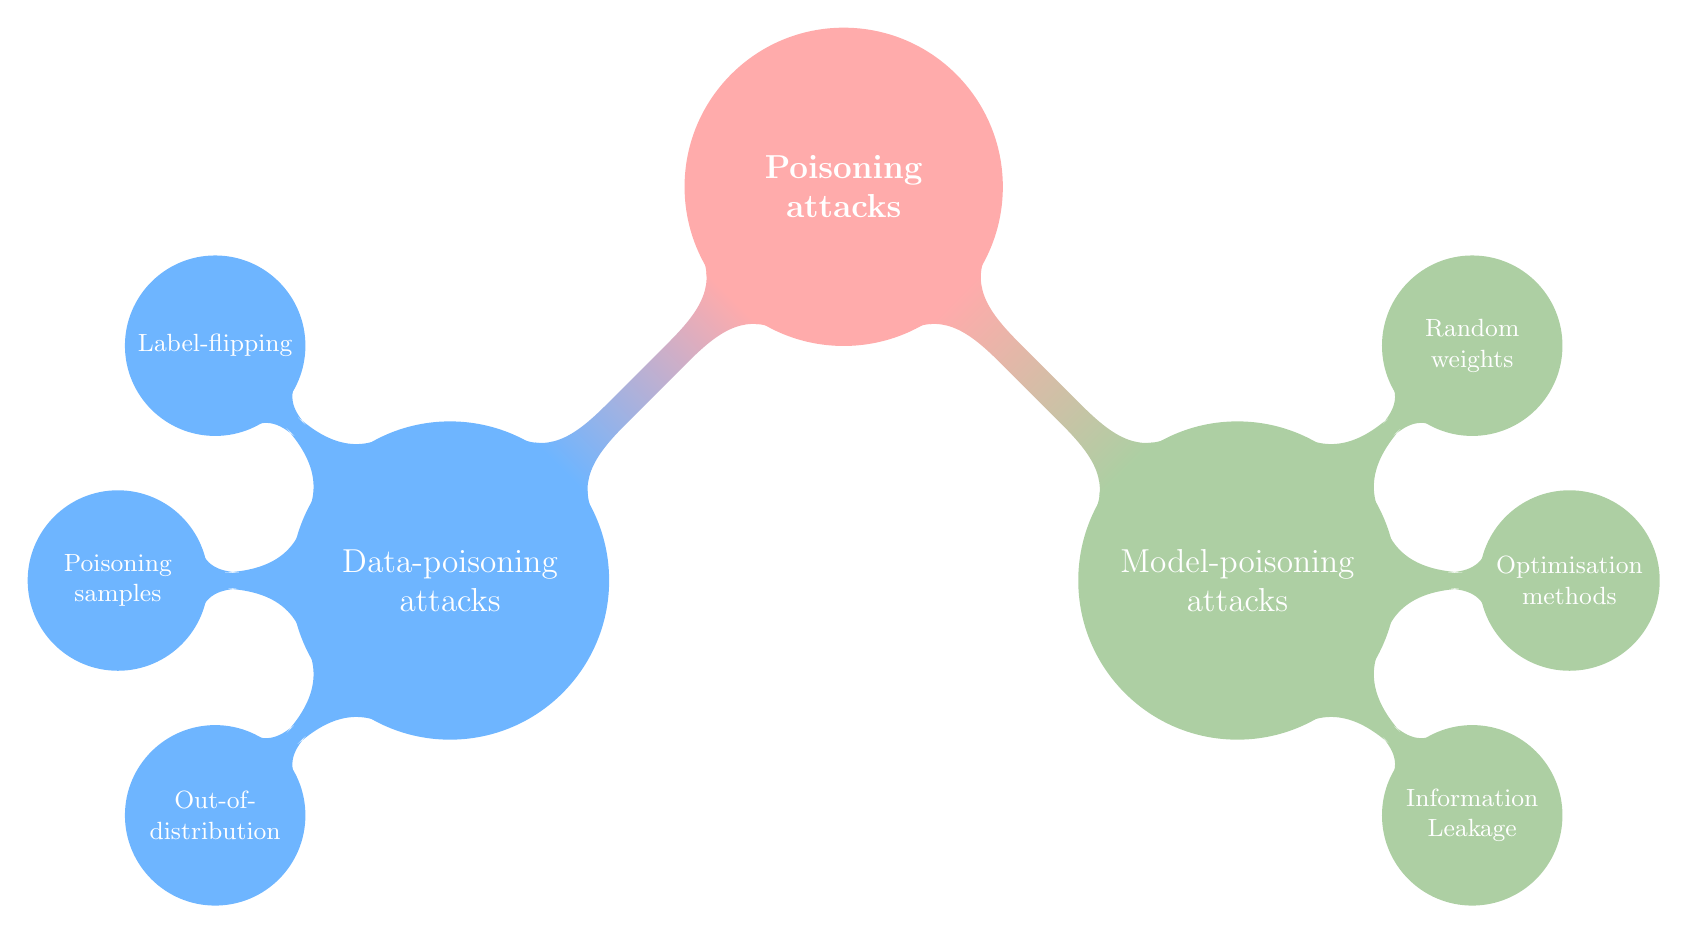
\begin{tikzpicture}[mindmap,
  level 1 concept/.append style={level distance=130,sibling angle=30},
  extra concept/.append style={color=blue!50,text=black}]

    \definecolor{rojo_pastel}{HTML}{FFABAB}
    \definecolor{azul_pastel}{HTML}{6EB5FF}
    \definecolor{verde_pastel}{HTML}{ADCFA3}
    \definecolor{morado_pastel}{HTML}{CAA7BD}

  \begin{scope}[mindmap, concept color=rojo_pastel, text=white]
    \node [concept] (root) at (0, 0) {\textbf{Poisoning attacks}};
  \end{scope}

  % Applied area: theoretical physics and its subfields

  \begin{scope}[mindmap, concept color=azul_pastel,text=white]
    \node [concept] (property) at (-5, -5) {Data-poisoning attacks}
        child [grow=135, level distance=120] {node [concept] (ind) {Label-flipping}}
        child [grow=180, level distance=120] {node [concept] (population) {Poisoning samples}}
        child [grow=225, level distance=120] {node [concept] (out-of) {Out-of-distribution}};
  \end{scope}
  
  
  \begin{scope}[mindmap, concept color=verde_pastel,text=white]
    \node [concept] (feature) at (5, -5) {Model-poisoning attacks}
        child [grow=45, level distance=120] {node [concept] (ind) {Random weights}}
        child [grow=0, level distance=120] {node [concept] (population) {Optimisation methods}}
        child [grow=-45, level distance=120] {node [concept] (out-of) {Information Leakage}};
  \end{scope}
  
  
    \path (root) to[circle connection bar switch color=from (rojo_pastel) to (azul_pastel)] (property);
    \path (root) to[circle connection bar switch color=from (rojo_pastel) to (verde_pastel)] (feature);

\end{tikzpicture}}
\end{center}
    \caption{Representación de la taxonomía según la parte del esquema envenenada. Fuente:~\cite{survey-nuria-2023}.}
    \label{fig:poisoned}
\end{figure}

\begin{itemize}
    \item \textbf{Ataques de Envenenamiento de Datos}: se asume que el atacante tiene acceso a los datos de entrenamiento de uno o más clientes y es capaz de modificarlos. Según las características del envenenamiento, podemos distinguir los siguientes ataques:
    \begin{itemize}
        \item \textbf{Ataque \textit{label-flipping}}: consiste en modificar las etiquetas de una parte del conjunto de datos. Puede ser con un objetivo, cambiando algunas etiquetas específicas, o sin objetivo, mediante barajando las etiquetas de manera aleatoria.
        \item \textbf{Ataque de envenenamiento de muestras}: este ataque consiste en modificar una parte de las muestras del conjunto de entrenamiento. El envenenamiento puede ser de distintos tipos, tales como añadir patrones en las muestras y asociarlos con una clase, o normalizar las muestras y añadir ruido uniforma con el objetivo de reducir el rendimiento del modelo.
        \item \textbf{Ataque fuera de distribución}: este ataque es similar al anterior, con la diferencia que las muestras envenenadas no son modificaciones de las originales sino muestras externas a la población original. Es posible usar muestras de otro dominio con las mismas características o muestras hechas por ruido aleatorio.
    \end{itemize}

    El objetivo de la mayoría de los ataques de envenenamiento de datos es reducir el rendimiento del modelo global y por tanto el modelo local de todos los clientes. Sin embargo, también existe el caso en el que el objetivo de los atacantes no es reducir el modelo global sino solo un subconjunto suyo. Es por ello por lo que podemos diferenciar tres tipos de ataques de envenenamiento de datos según el nivel de acceso que los atacantes tienen sobre los nodos objetivo:
    \begin{itemize}
        \item \textbf{Ataque directo}: los atacantes tienen acceso a los nodos objetivo, así que los envenenan directamente.
        \item \textbf{Ataque indirecto}: los atacantes no tienen acceso a los nodos objetivo, así que aplican mecanismos tales como entrenar sus propios modelos con datos envenenados para envenenar el modelo global, que luego será compartido con los nodos objetivo.
        \item \textbf{Ataque híbrido}: cuando se combinan ambos ataques mencionados.
    \end{itemize}

    En la literatura los ataques más comunes son los ataques directos.
    \item \textbf{Ataques de Envenenamiento de Modelo}: estos ataques consisten en envenenar directamente las actualizaciones del modelo que son mandadas por los clientes al servidor. Pese a que los ataques de envenenamiento de datos llevan a ataques de envenenamiento de modelo, nos centraremos en aquellos ataques que modifican directamente las actualizaciones locales. Según cómo son generadas, distinguimos entre:
    \begin{itemize}
        \item \textbf{Generación de pesos aleatorios}: estos ataques se basan en generar pesos del modelo como un vector de la misma dimensión que los pesos del servidor generado aleatoriamente.
        \item \textbf{Métodos de optimización}: consisten en maximizar el rendimiento en una tarea de \textit{backdoor}, mientras se minimizan las diferencias del modelo envenenado respecto al compartido con el servidor en la última ronda, maximizando así la efectividad y sigilo. Este ataque se realiza como un problema de optimización multiobjetivo. Este tipo de ataque es posiblemente el más eficaz para realizar ataques de \textit{backdoor} en el modelo.
        \item \textbf{Brecha de información}: un caso particular de los ataques de envenenamiento de modelo es la brecha de información, donde el objetivo no es perjudicar al modelo global, sino la comunicación entre los atacantes a través de un protocolo seguro. Consiste en que varios clientes están coordinados dde tal manera que conocen reglas comunes y mediante la modificación de pequeñas partes de los pesos del modelo pueden comunicarse.
    \end{itemize}
\end{itemize}

En el \ac{FL}, asumiendo que la proporción de clientes adversarios es significativamente inferior a la de los benignos, el efecto del ataque se espera que sea disipado en el proceso de agregación. Por lo tanto, se aplican técnicas de \textit{model-replacement}, que consisten en ponderar la contribución de los clientes adversarios usando técnicas de \textit{boosting} con el objetivo de reemplazar el modelo agregado con sus actualizaciones locales. Formalmente, si consideramos la actualización del modelo global en la ronda $t$ se computa según \eqref{fedavg}:
\begin{equation}\label{fedavg}
    G^t = G^{t-1} + \frac{\eta}{n}\sum^n_{i=1}(L^t_i - G^{t-1})
\end{equation}

donde $\eta$ es el \textit{learning rate} del servidor y $n$ la cantidad de clientes participando en la agregación. Entonces consideramos el modelo local del cliente adversario entrenado en los datos envenenados como en \eqref{modelreplacementupdate}:
\begin{equation}\label{modelreplacementupdate}
    \hat{L}^t_{adv} = \beta(L^t_{adv} - G^{t-1})
\end{equation}

donde $\beta=\frac{n}{\eta}$ es el factor de \textit{boosting}. Combinando entonces \eqref{fedavg} y \eqref{modelreplacementupdate} tenemos\footnote{Asumimos que el adversario es el cliente 1} que:
\begin{equation}\label{modelreplacementfull}
    G^t = G^{t-1} = \frac{\eta}{n}\frac{n}{\eta}(L^t_{adv} - G^{t-1}) + \frac{\eta}{n}\sum_{i=2}^n(L^t_i - G^{t-1})
\end{equation}
Además, debido a que el modelo de \ac{FL} convergerá a una solución, se puede asumir que $L^t_i - G^{t-1} \approx 0$ para los clientes benignos. Por lo tanto se puede reescribir \eqref{modelreplacementfull} como:
\begin{equation}
    G^t \approx G^{t-1} + \frac{\eta}{n}\frac{n}{\eta}(L^t_{adv} - G^{t-1}) = L^t_{adv}
\end{equation}

Si hay varios clientes adversarios, el factor de \textit{boosting} se divide entre todos ellos.

Las técnicas de \textit{boosting} dependen de saber el número de clientes participando en la agregación, lo cuál es una condición mucho más restrictiva de conocimiento por parte del cliente. En la práctica, el cliente estima este valor haciendo varias pruebas con distintos valores y analizando las actualizaciones devueltas por el servidor. Sin embargo, en la mayoría de trabajos experimentales se asume la peor situación en la que este conocimiento es sabido.

\paragraph{Taxonomía según la frecuencia}\mbox{}\\

Debido a que el entrenamiento ocurre durante un periodo prolongado en el tiempo, los ataques durante entrenamiento pueden ser realizados en cualquier momento durante el entrenamiento y en una o varias ocasiones. Diferenciamos entre dos categorías:
\begin{itemize}
    \item \textbf{Ataque \textit{One-shot}}: este ataque es realizado en un único momento durante el entrenamiento, en una ronda de aprendizaje en específico.
    \item \textbf{Ataque Múltiple o Adaptativo}: los ataques se realizan de manera continua durante el proceso de entrenamiento, ya sea durante todas las rondas de aprendizaje o sobre una porción de ellas.
\end{itemize}

\section{Métodos de Defensa contra Ataques Adversarios}
Mientras que la diversidad y la complejidad de los ataques adversarios contra el \ac{FL} está aumentando, aparecen nuevas defensas para mitigar sus efectos maliciosos. Aunque los ataques adversarios pueden ser divididos en categorías disjuntas, esto no se cumple para sus defensas ya que algunas son efectivas contra más de un tipo de ataque. Por lo tanto, en lugar de agrupar las defensas según el ataque contra el que defienden, \cite{survey-nuria-2023} propone categorizarlas en tres grupos según el esquema federado en el que se implementan: el cliente, el servidor o el canal de comunicación.

\begin{figure}[!t]
\centering
\usetikzlibrary{mindmap,backgrounds}

\begin{center}
\resizebox{0.8\textwidth}{!}{
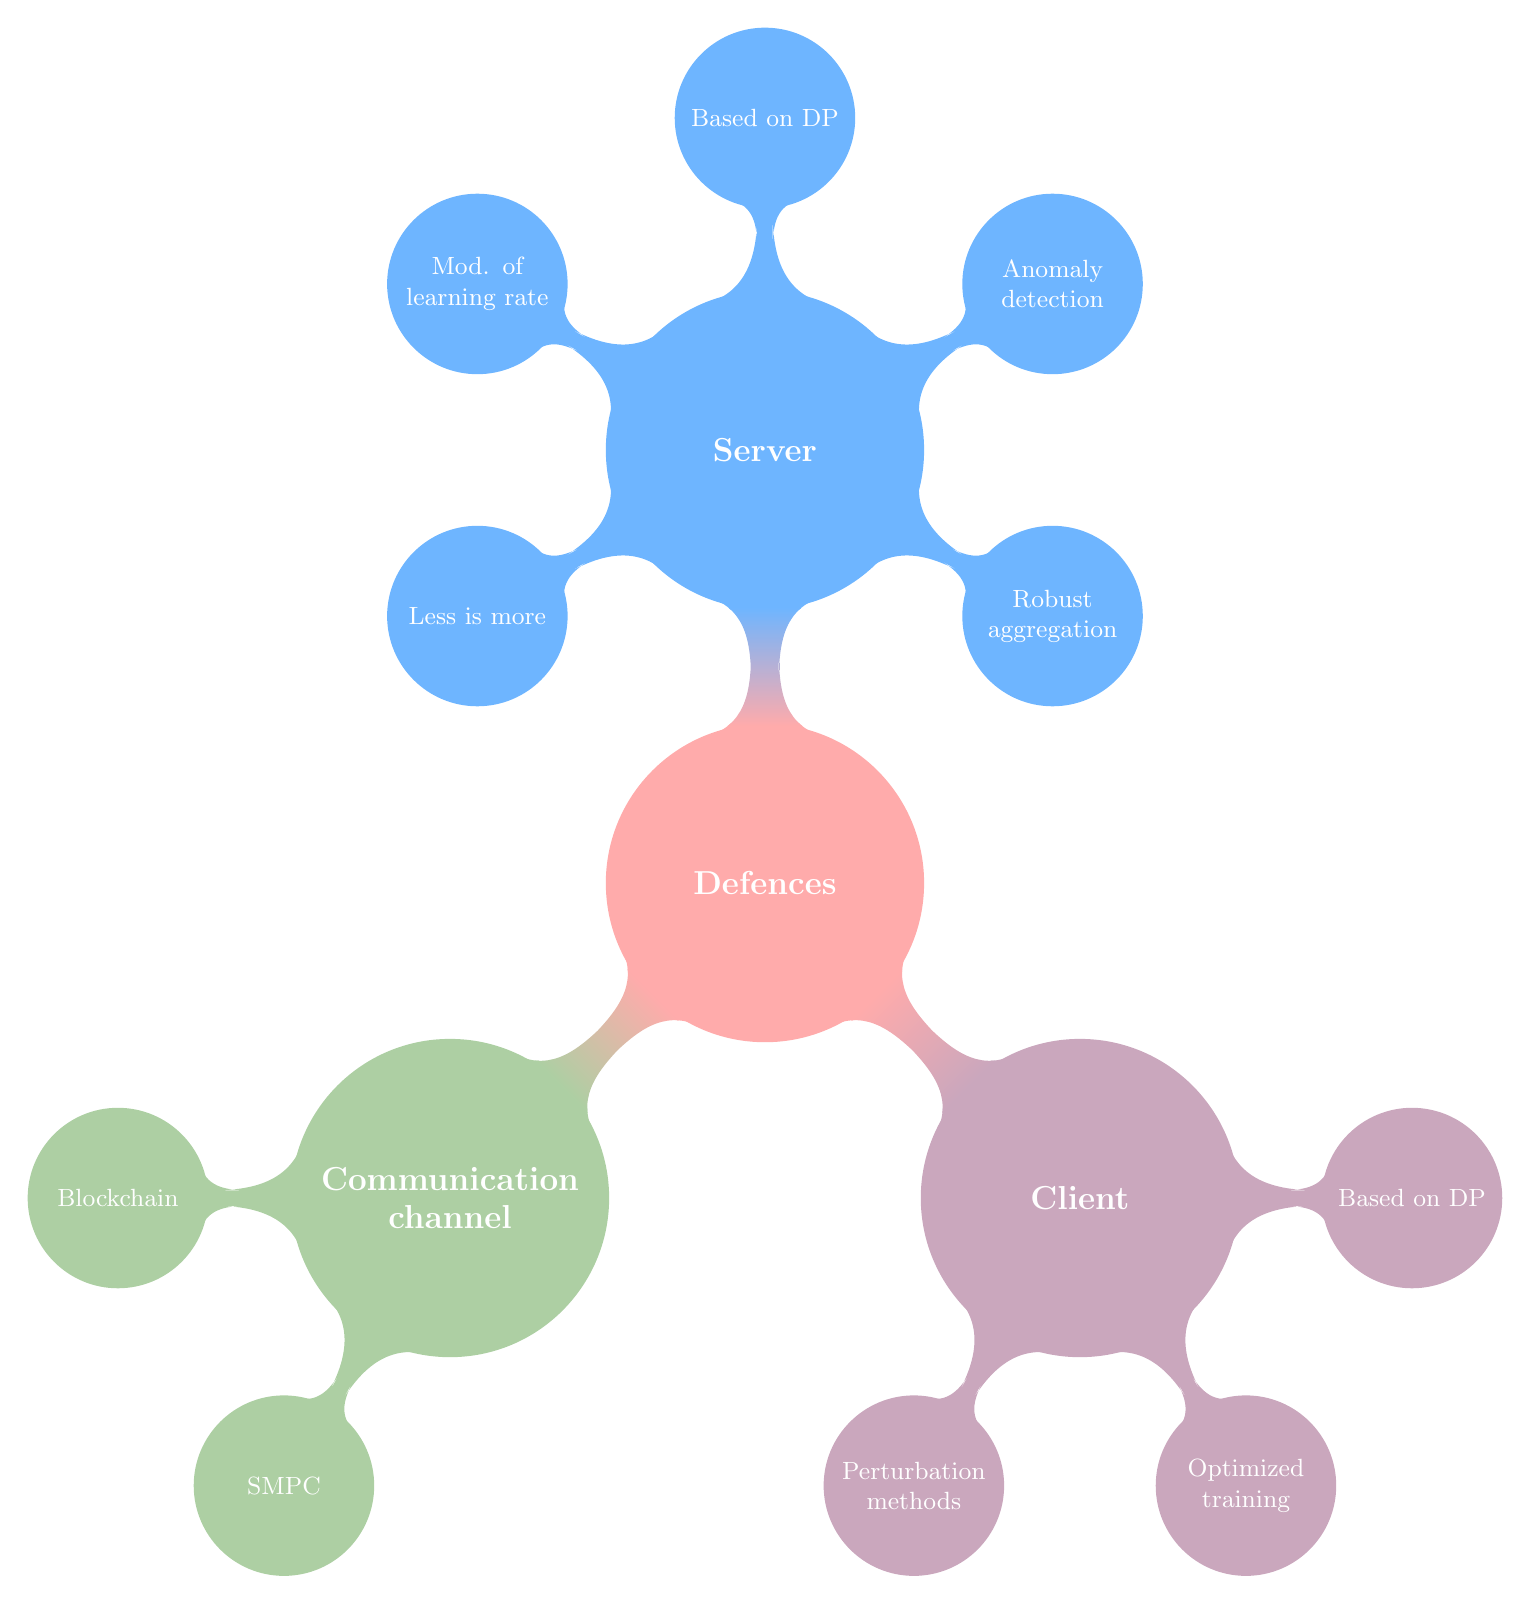
\begin{tikzpicture}[mindmap,
  level 1 concept/.append style={level distance=130,sibling angle=30},
  extra concept/.append style={color=verde_pastel!50,text=black}]

    \definecolor{rojo_pastel}{HTML}{FFABAB}
    \definecolor{azul_pastel}{HTML}{6EB5FF}
    \definecolor{verde_pastel}{HTML}{ADCFA3}
    \definecolor{morado_pastel}{HTML}{CAA7BD}
  % Applied area: computer science and its subfields

  \begin{scope}[mindmap, concept color=rojo_pastel, text=white]
    \node [concept] (def) at (0, 0) {\textbf{Defences}};
  \end{scope}
  
    \begin{scope}[mindmap, concept color=azul_pastel, text=white]
    \node [concept] (ser) at (0, 5.5) {\textbf{Server}}
        child [grow=-30, level distance=120] {node [concept] {Robust aggregation}}
        child [grow=30, level distance=120] {node [concept] {Anomaly detection}}
        child [grow=90, level distance=120] {node [concept] {Based on DP}}
        child [grow=150, level distance=120] {node [concept] {Mod. of learning rate}}
        child [grow=210, level distance=120] {node [concept] {Less is more}};
  \end{scope}
  
    \begin{scope}[mindmap, concept color=verde_pastel, text=white]
    \node [concept] (cli) at (-4, -4) {\textbf{Communication channel}}
        child [grow=180, level distance=120] {node [concept] {Blockchain}
      }
      child [grow=240, level distance=120] {node [concept] {SMPC}};
  \end{scope}
  
    \begin{scope}[mindmap, concept color=morado_pastel, text=white]
    \node [concept] (com) at (4, -4) {\textbf{Client}}
      child [grow=0, level distance=120] {node [concept] {Based on DP}}
      child [grow=-120, level distance=120] {node [concept] {Perturbation methods}}
      child [grow=-60, level distance=120] {node [concept] {Optimized training}};
  \end{scope}
  
    \path (def) to[circle connection bar switch color=from (rojo_pastel) to (azul_pastel)] (ser);
    \path (def) to[circle connection bar switch color=from (rojo_pastel) to (verde_pastel)] (cli);
    \path (def) to[circle connection bar switch color=from (rojo_pastel) to (morado_pastel)] (com);



\end{tikzpicture}}
\end{center}
\caption{Representación de la taxonomía de las defensas contra ataques adversarios. Fuente:~\cite{survey-nuria-2023}.}
\label{fig:defences}
\end{figure}

\subsection{Defensas en el Servidor}
Normalmente se asume que se puede confiar en el servidor, ya que es un elemento federado controlado y accesible por expertos en \ac{FL}, al contrario que los clientes que son elementos independientes e inaccesibles. Por lo tanto, la mayor parte de las defensas son implementadas en el servidor. Dentro de este tipo de defensas, se presenta la siguiente taxonomía. Debemos de tener en cuenta que algunas defensas pueden tener elementos de más de una categoría , aunque dada una defensa esta se ha clasificado en la categoría que mejor la representa según \cite{survey-nuria-2023}.

\paragraph{Operadores Robustos de Agregación}\mbox{}\\
La técnica más común para defenderse ante ataques de envenenamiento es el usar estimadores que sean más robustos que la media a \textit{outliers} o valores extremos, desde un punto de vista estadístico. Algunos agregadores, como \ac{FedAvg}~\cite{mcmahan-2023}, son sensibles a \textit{outliers}. Es por esta razón que se han propuesto muchos operadores de agregación basados en estimadores más robustos. Pueden destacarse los siguientes:
\begin{itemize}
    \item \textit{Mediana:} se basa en reemplazar la media aritmética por la mediana de las actualizaciones de los modelos.
    \item \textit{Media Geométrica:} representa la tendencia central o el valor típico de la distribución mediante el uso del producto de sus valores. Se puede decir que escoge un vector que representa las actualizaciones de los modelos locales mediante voto de la mayoría.
    \item \textit{Krum y Multikrum \cite{krum-2017}:} este agregador está diseñado para prevenir ataques al modelo federado. Consiste en filtrar las actualizaciones que representan un comportamiento externo. Para ello se ordenan los clientes según las distancias geométricas de sus distribuciones y se escoge la más cercana a la mayoría como modelo agregado. Multikrum incorpora un parámetro que especifica la cantidad de clientes a ser agregados.
    \item \textit{Bulyan:} pensado para evitar ataques de envenenamiento, combina el operador de Multikrum con la media recortada.
\end{itemize}

\paragraph{Detección de Anomalías}\mbox{}\\
Estos métodos de defensa consisten en identificar clientes adversarios mediante datos anómalos en la distribución y retirarlos de la agregación. Para este propósito, se aplican técnicas de detección de anomalías multivariante o univariante en \ac{AA}.

Uno de los mecanismos propuestos es \textit{AUROR}, un mecanismo contra ataques de envenenamiento basado en \textit{K-Means} con $k=2$, por lo tanto distinguiendo entre \textit{clusters} benignos y maliciosos. El principal problema de esta propuesta es que si se da la presencia de distribuciones no-\ac{i.i.d.} entre los clientes podría fallar a la hora de identificar los \textit{clusters}.

El principal problema con técnicas de detección de anomalías es que las actualizaciones del modelo tienden a ser de una dimensión muy alta, ya que vienen de redes neuronales la mayoría de ocasiones. Es por ello que aparecen varias propuestas que intentan reducir la dimensionalidad de las datos ya sea basándose en análisis de componentes principales o en técnicas similares, aunque conllevan también una pérdida de información en el proceso.

\paragraph{Defensas Basadas en Privacidad Diferencial}\mbox{}\\
Aunque la privacidad es algo que se escapa a los ataques adversarios al modelo, la \ac{DP} ha demostrado ser una defensa viable contra este tipo de ataques. Sin embargo, también se sabe que la \ac{DP} puede impactar negativamente al rendimiento de los modelos bajo circunstancias de un desequilibrio en las distribuciones datos, que es lo esperado a ocurrir en la mayoría de escenarios federados.

\paragraph{Modificación del \textit{Learning Rate}}\mbox{}\\
Una de las ventajas del servidor es que es él el que establece el peso entre la versión previa del modelo y de las actualizaciones de los modelos locales según 
\begin{equation}
    G^t = G^{t-1} + \eta \Delta(L^t_1, \ldots, L^t_n)
\end{equation}

donde $G^t$ es el modelo global en la ronda $t$, $\eta$ es el \ac{lr}, $\Delta$ el operador de agregación y $L_i^t$ las actualizaciones del cliente $i$ en la ronda $t$. Otra posibilidad es la de descomponer $\eta$ en un vector de \ac{lr} con una componente por cada dimensión. Por lo tanto en servidor controla la participación de cada dimensión en las actualizaciones del modelo. 

Se propone \textit{Robust Learning Rate} como un mecanismo de defensa basado en ajustar el \ac{lr} del servidor, por dimensión, en cada ronda de aprendizaje según la información de las actualizaciones de los clientes. Para cada dimensión, se examina si los clientes acuerdan la dirección de las actualizaciones usando algún tipo de umbral predefinido. Si el acuerdo es mayor que el requerido por el umbral, se mantiene el \ac{lr}, en caso contrario se cambia el signo del \ac{lr}.

\subsection{Defensas en el Cliente}
Las defensas en el servidor asumen que el servidor es un recolector de datos y un agregador fiable. Sin embargo, asumir esto puede ser demasiado, por lo tanto hay una necesidad de defensas cuando no asumimos un servidor fiable. En esta situación se despliegan defensas en el cliente y por lo tanto, al menos una parte de los clientes se supone que es benigna. Si bien las defensas en el servidor protegían a los clientes como conjunto, estas se consideran más fuertes pues defienden a cada cliente individualmente.

\paragraph{Basadas En Privacidad Diferencial}\label{sec:fldp}\mbox{}\\
Generalmente, este tipo de defensas están pensadas para defenderse contra ataques de privacidad en el servidor, aunque pueden proteger a los clientes de ataques adversarios. La \ac{DP} local es la principal defensa basada en \ac{DP} en el cliente. Por lo tanto muchos autores han propuesto mejor a la \ac{DP} local mediante la disminución de su uso, es decir, usando el menor ruido necesario. Se ha estudiado su efectividad contra ataques adversarios y se ha relacionado el impacto negativo al rendimiento de esta técnica con la reducción de la efectividad del ataque adversario.


\paragraph{Métodos de Perturbación}\mbox{}\\
Son una técnica alternativa a la \ac{DP} para defenderse contra ataques a la privacidad. Su principal objetivo es el introducir ruido a las partes más vulnerables del modelo federado, tales como los parámetros compartidos o al conjunto de datos local de cada cliente, para reducir la cantidad de información que el atacante puede extraer. Algunos trabajos proponen podar los gradientes que estén por debajo de cierto umbral o perturbar los datos locales de los clientes con una red neuronal.

\paragraph{Entrenamiento Optimizado}\mbox{}\\
La optimización del entrenamiento de los clientes benignos puede ser un método para proteger al sistema federado de ataques adversarios. Por ejemplo, se propone realizar \textit{fine-tuning} del modelo en los clientes benignos con el objetivo de aumentar el impacto de estos clientes en la agregación. Para decir que clientes son benignos, se hace uso de \textit{matching networks}, que consiste en medir la similitud entre las actualizaciones de los modelos y el modelo anterior. En casos experimentales, se logra filtrar tareas de \textit{backdoor} aunque conlleva un impacto negativo en el rendimiento de la tarea original.

\subsection{Defensas en el Canal de Comunicación}
Estas defensas permiten a varios clientes realizar una tarea global, asumiendo la presencia de actores maliciosos que intentan perjudicar a la tarea. Estos actores pueden ser vistos como los atacantes en nuestro caso, que intentan realizar algún tipo de ataque adversario mencionado previamente. Mientas que se mantiene la privacidad de los datos usados para realizar la tarea global, el resultado de esta se revela a algunos grupos, sino a todos. Por lo tanto la privacidad del resultado no está asegurada, aunque se detienen algunos ataques de privacidad ya que el atacante pierde acceso a los resultados intermedios de la tarea global tales como parámetros o gradientes usados por los clientes.

\paragraph{Federated Learning basado en Blockchain}\mbox{}\\
Esta será la defensa más importante de nuestro trabajo y en la que nos centraremos más adelante en este trabajo en los próximos capítulos. La tecnología \textit{Blockchain} permite un esquema de \ac{FL} descentralizado sin riesgos de un único punto de fallo y una escalabilidad mejorada. Aún así también implica algunos riesgos inherentes a las \textit{Blockchain} como ataques del 51\% o ataques de \textit{forking} entre otros. Sin embargo veremos más adelante como pueden ser realmente útiles como defensas ante ataques adversarios al modelo.